\documentclass[ignorenonframetext,]{beamer}
\setbeamertemplate{caption}[numbered]
\setbeamertemplate{caption label separator}{:}
\setbeamercolor{caption name}{fg=normal text.fg}
\usepackage{amssymb,amsmath}
\usepackage{ifxetex,ifluatex}
\usepackage{fixltx2e} % provides \textsubscript
\usepackage{lmodern}
\ifxetex
  \usepackage{fontspec,xltxtra,xunicode}
  \defaultfontfeatures{Mapping=tex-text,Scale=MatchLowercase}
  \newcommand{\euro}{€}
\else
  \ifluatex
    \usepackage{fontspec}
    \defaultfontfeatures{Mapping=tex-text,Scale=MatchLowercase}
    \newcommand{\euro}{€}
  \else
    \usepackage[T1]{fontenc}
    \usepackage[utf8]{inputenc}
      \fi
\fi
% use upquote if available, for straight quotes in verbatim environments
\IfFileExists{upquote.sty}{\usepackage{upquote}}{}
% use microtype if available
\IfFileExists{microtype.sty}{\usepackage{microtype}}{}
\usepackage{color}
\usepackage{fancyvrb}
\newcommand{\VerbBar}{|}
\newcommand{\VERB}{\Verb[commandchars=\\\{\}]}
\DefineVerbatimEnvironment{Highlighting}{Verbatim}{commandchars=\\\{\}}
% Add ',fontsize=\small' for more characters per line
\newenvironment{Shaded}{}{}
\newcommand{\KeywordTok}[1]{\textcolor[rgb]{0.26,0.66,0.93}{\textbf{{#1}}}}
\newcommand{\DataTypeTok}[1]{\underline{{#1}}}
\newcommand{\DecValTok}[1]{\textcolor[rgb]{0.27,0.67,0.26}{{#1}}}
\newcommand{\BaseNTok}[1]{\textcolor[rgb]{0.27,0.67,0.26}{{#1}}}
\newcommand{\FloatTok}[1]{\textcolor[rgb]{0.27,0.67,0.26}{{#1}}}
\newcommand{\CharTok}[1]{\textcolor[rgb]{0.02,0.61,0.04}{{#1}}}
\newcommand{\StringTok}[1]{\textcolor[rgb]{0.02,0.61,0.04}{{#1}}}
\newcommand{\CommentTok}[1]{\textcolor[rgb]{0.00,0.40,1.00}{\textit{{#1}}}}
\newcommand{\OtherTok}[1]{{#1}}
\newcommand{\AlertTok}[1]{\textcolor[rgb]{1.00,1.00,0.00}{{#1}}}
\newcommand{\FunctionTok}[1]{\textcolor[rgb]{1.00,0.58,0.35}{\textbf{{#1}}}}
\newcommand{\RegionMarkerTok}[1]{{#1}}
\newcommand{\ErrorTok}[1]{\textbf{{#1}}}
\newcommand{\NormalTok}[1]{{#1}}
\usepackage{graphicx}
\makeatletter
\def\maxwidth{\ifdim\Gin@nat@width>\linewidth\linewidth\else\Gin@nat@width\fi}
\def\maxheight{\ifdim\Gin@nat@height>\textheight0.8\textheight\else\Gin@nat@height\fi}
\makeatother
% Scale images if necessary, so that they will not overflow the page
% margins by default, and it is still possible to overwrite the defaults
% using explicit options in \includegraphics[width, height, ...]{}
\setkeys{Gin}{width=\maxwidth,height=\maxheight,keepaspectratio}

% Comment these out if you don't want a slide with just the
% part/section/subsection/subsubsection title:
\AtBeginPart{
  \let\insertpartnumber\relax
  \let\partname\relax
  \frame{\partpage}
}
\AtBeginSection{
  \let\insertsectionnumber\relax
  \let\sectionname\relax
  \frame{\sectionpage}
}
\AtBeginSubsection{
  \let\insertsubsectionnumber\relax
  \let\subsectionname\relax
  \frame{\subsectionpage}
}

\setlength{\parindent}{0pt}
\setlength{\parskip}{6pt plus 2pt minus 1pt}
\setlength{\emergencystretch}{3em}  % prevent overfull lines
\setcounter{secnumdepth}{0}
\usepackage{svg}
\usepackage{amsmath}
\usepackage{tikz}
\usetikzlibrary{shapes.arrows}
\usepackage[normalem]{ulem}
\usetheme{Warsaw}
\beamertemplatenavigationsymbolsempty
\setbeamertemplate{footline}[frame number]
\usefonttheme{structurebold}

\setbeamertemplate{itemize items}[default]
\setbeamertemplate{enumerate items}[default]

\setbeamercolor{normal text}{fg=white,bg=black!95}
\setbeamercolor{structure}{fg=white}

\setbeamercolor{alerted text}{fg=red!60!white}

\setbeamercolor{item projected}{use=item,fg=black,bg=item.fg!35}

\definecolor{BlueLike}{RGB}{83,121,170}
\definecolor{BlueDifferentLike}{RGB}{93,106,251}
\definecolor{Carrot}{RGB}{255,137,67}
\definecolor{Rounge}{RGB}{255,102,0}
\definecolor{Pinkish}{RGB}{201,124,204}

\setbeamercolor{title}{fg=BlueDifferentLike}
\setbeamercolor{structure}{fg=Rounge}

\setbeamercolor*{palette primary}{use=structure,fg=structure.fg}
\setbeamercolor*{palette secondary}{use=structure,fg=structure.fg!95!black}
\setbeamercolor*{palette tertiary}{use=structure,fg=structure.fg!90!black}
\setbeamercolor*{palette quaternary}{use=structure,fg=structure.fg!95!black,bg=black!80}

\setbeamercolor*{framesubtitle}{fg=white}

\setbeamercolor*{block title}{parent=structure,bg=black!60}
\setbeamercolor*{block body}{fg=black,bg=black!10}
\setbeamercolor*{block body alerted}{fg=black,bg=red!20!white}
\setbeamercolor*{block title alerted}{fg=white,bg=red!80}

\tikzset{
    myarrow/.style={
        draw,
        fill=black,
        single arrow,
        minimum height=3.5ex,
        single arrow head extend=1ex
    }
}
\newcommand{\arrowup}{%
\tikz [baseline=-0.5ex]{\node [myarrow,rotate=90] {};}
}
\newcommand{\arrowdown}{%
\tikz [baseline=-1ex]{\node [myarrow,rotate=-90] {};}
}

\inputencoding{utf8}
\usepackage[orientation=landscape,size=custom,width=16,height=9,scale=0.5,debug]{beamerposter}

\title{Your Web Service as a Type}
\author{(Typing REST APIs with Servant)}
\date{}

\begin{document}
\frame{\titlepage}

\begin{frame}{Every time we write a REST API}

Your API will\ldots{}

\begin{itemize}[<+->]
\itemsep1pt\parskip0pt\parsep0pt
\item
  Explode in subtle ways
\item
  Boilerplate gets mixed with important business logic
\item
  Complexity becomes nightmare to maintain
\item
  Becomes partially and/or inconsistently documented
\end{itemize}

\end{frame}

\begin{frame}{Servant is\ldots{}}

\begin{itemize}[<+->]
\itemsep1pt\parskip0pt\parsep0pt
\item
  A collection of libraries built around the concept of typed APIs.
\item
  n devs
\item
  n commercial users
\item
  About to hit a 0.3 release with some major improvements.
\end{itemize}

\end{frame}

\begin{frame}{Your API wants types}

\begin{columns}

\column{0.5\textwidth}

\emph{REST problems}

\begin{itemize}[<+->]
\itemsep1pt\parskip0pt\parsep0pt
\item
  Explode in subtle ways
\item
  Boilerplate gets mixed with important business logic
\item
  Complexity becomes nightmare to maintain
\item
  Becomes partially and/or inconsistently documented
\end{itemize}

\column{0.5\textwidth}

\emph{Types can fix that!}

\begin{itemize}[<+->]
\itemsep1pt\parskip0pt\parsep0pt
\item
  Explode in obvious ways
\item
  Make generic programming an option
\item
  Provide a framework for complexity
\item
  Provide documentation, with 100\% coverage
\end{itemize}

\end{columns}

\end{frame}

\begin{frame}{How do you even?}

How do we represent our API as a type?

First, let's look at it like a tree:

\begin{itemize}[<+->]
\itemsep1pt\parskip0pt\parsep0pt
\item
  Leaves are endpoints (GET, POST, etc)
\item
  Nodes along the way to leaves ``modify'' that endpoint.
\end{itemize}

\end{frame}

\begin{frame}{APIs have shapes}

\begin{figure}[htbp]
\centering
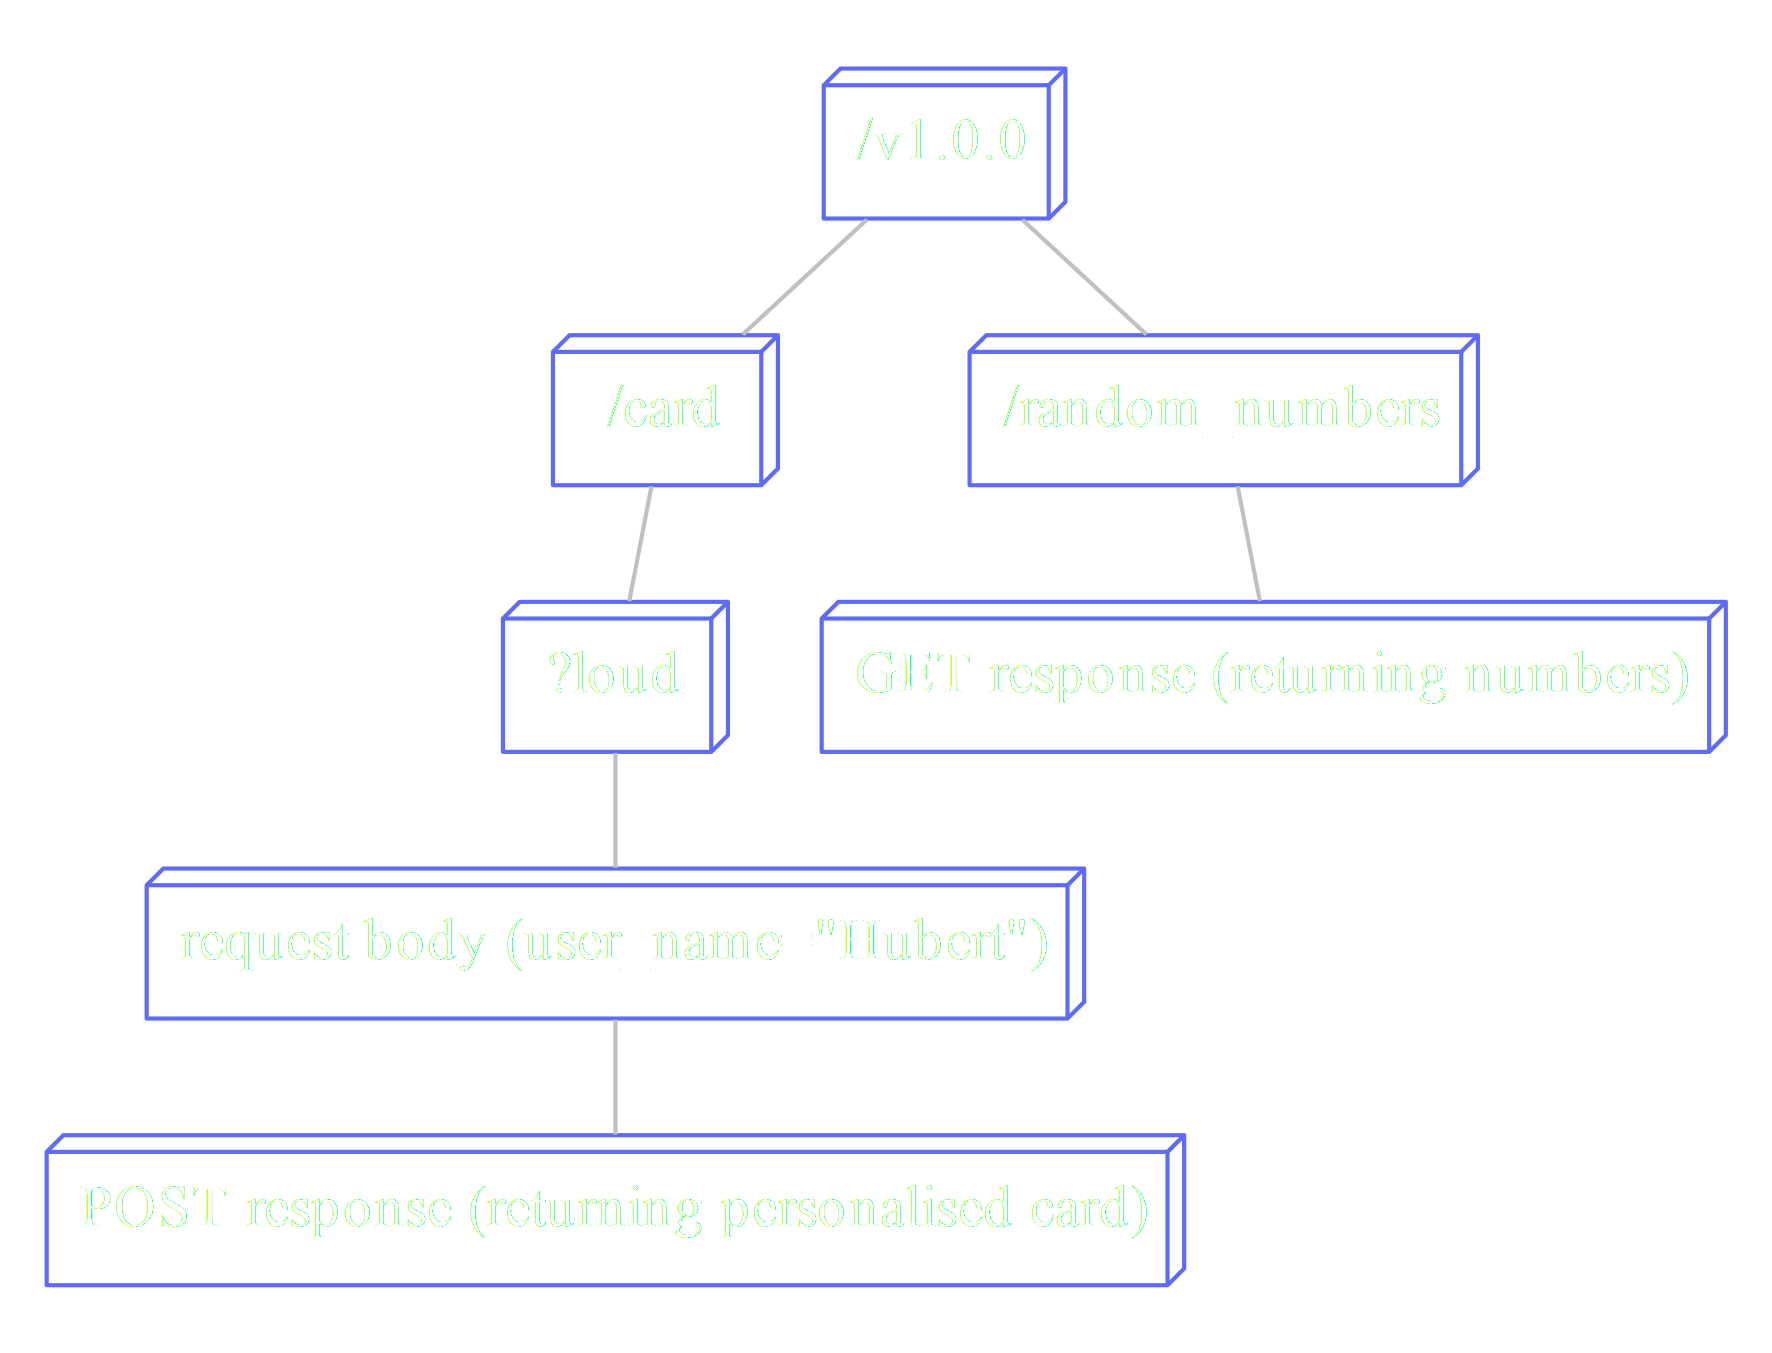
\includegraphics{tree.png}
\caption{Your API as a tree}
\end{figure}

\end{frame}

\begin{frame}[fragile]{Types have shapes (type operators)}

\begin{columns}

\column{0.5\textwidth}

\emph{head :\textgreater{} tail}

\begin{itemize}[<+->]
\itemsep1pt\parskip0pt\parsep0pt
\item
  For joining nodes
\item
  Constructor for a type level non-empty list
\item
  Not directly inhabitable
\end{itemize}

\column{0.5\textwidth}

\emph{branch1 :\textless{}\textbar{}\textgreater{} branch2}

\begin{itemize}[<+->]
\itemsep1pt\parskip0pt\parsep0pt
\item
  For branching
\item
  Constructor for alternatives (disjunction)
\item
  Inhabitable via :\textless{}\textbar{}\textgreater{}
\end{itemize}

\end{columns}

\begin{columns}

\column{0.5\textwidth}

\begin{Shaded}
\begin{Highlighting}[]
\KeywordTok{data} \NormalTok{(}\OtherTok{path ::} \NormalTok{k) }\FunctionTok{:>} \NormalTok{a}
    \KeywordTok{deriving} \NormalTok{(}\DataTypeTok{Typeable}\NormalTok{)}
    \KeywordTok{infixr} \DecValTok{9} \FunctionTok{:>}
\end{Highlighting}
\end{Shaded}

\column{0.5\textwidth}

\begin{Shaded}
\begin{Highlighting}[]
\KeywordTok{data} \NormalTok{a }\FunctionTok{:<|>} \NormalTok{b }\FunctionTok{=} \NormalTok{a }\FunctionTok{:<|>} \NormalTok{b}
    \KeywordTok{deriving} \NormalTok{(}\DataTypeTok{Typeable}\NormalTok{, }\DataTypeTok{Eq}\NormalTok{, }\DataTypeTok{Show}\NormalTok{)}
\KeywordTok{infixr} \DecValTok{8} \FunctionTok{:<|>}
\end{Highlighting}
\end{Shaded}

\end{columns}

\end{frame}

\begin{frame}{APIs have shapes}

\begin{figure}[htbp]
\centering
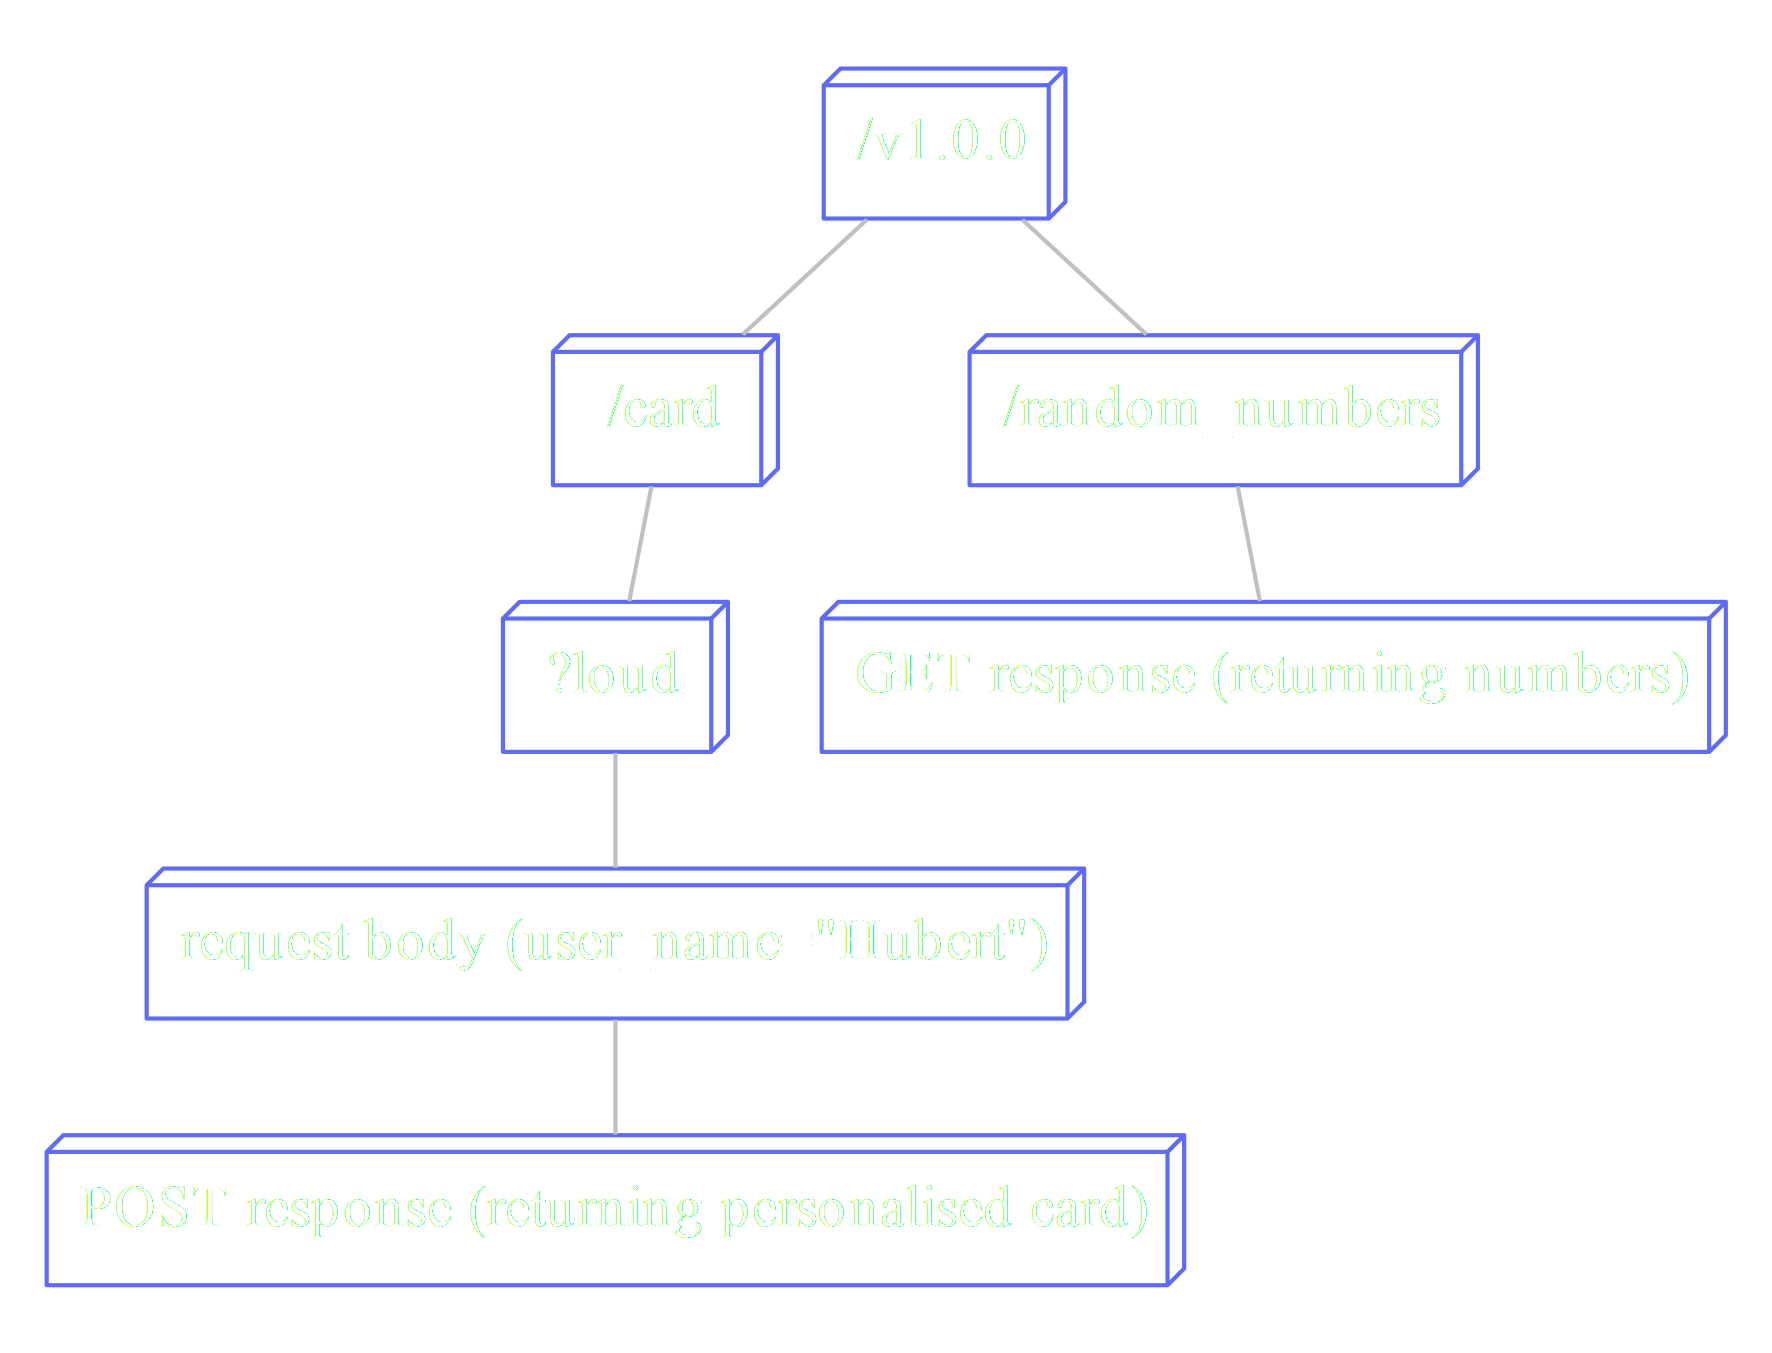
\includegraphics{tree.png}
\caption{Your API as a tree}
\end{figure}

\end{frame}

\begin{frame}[fragile]{Shape as a type!}

\begin{Shaded}
\begin{Highlighting}[]

\KeywordTok{type} \DataTypeTok{MakeCard} \FunctionTok{=}
    \StringTok{"card"}
    \FunctionTok{:>} \DataTypeTok{QueryFlag} \StringTok{"loud"}
    \FunctionTok{:>} \DataTypeTok{ReqBody} \CharTok{'[FormUrlEncoded, JSON] Name}
    \FunctionTok{:>} \DataTypeTok{Post} \CharTok{'[JSON] PersonalisedCard}

\KeywordTok{type} \DataTypeTok{RandomInt} \FunctionTok{=}
    \StringTok{"random_number"} \FunctionTok{:>} \DataTypeTok{Get} \CharTok{'[JSON] Int}

\KeywordTok{type} \DataTypeTok{CardAPI} \FunctionTok{=} \StringTok{"v1.0.0"} \FunctionTok{:>} \NormalTok{(}\DataTypeTok{MakeCard} \FunctionTok{:<|>} \DataTypeTok{RandomInt}\NormalTok{)}
\end{Highlighting}
\end{Shaded}

\end{frame}

\begin{frame}{How would a typed API even work?}

Before we can type the APIs, I have to explain some ``fundamentals'':

\begin{itemize}[<+->]
\itemsep1pt\parskip0pt\parsep0pt
\item
  DataKinds
\item
  PolyKinds
\item
  Data.Proxy
\item
  GHC.TypeLits
\item
  TypeFamilies
\end{itemize}

\end{frame}

\begin{frame}[fragile]{DataKinds, PolyKinds, Proxy \& TypeLits}

\begin{Shaded}
\begin{Highlighting}[]
\KeywordTok{import }\DataTypeTok{Data.Proxy}
\KeywordTok{import }\DataTypeTok{GHC.TypeLits}

\CommentTok{-- | A concrete, poly-kinded proxy type  }
\KeywordTok{data} \DataTypeTok{Proxy} \NormalTok{a }\FunctionTok{=} \DataTypeTok{Proxy}

\OtherTok{stringProxy ::} \DataTypeTok{Proxy} \StringTok{"I AM A TYPE-LEVEL STRING!"}
\NormalTok{stringProxy }\FunctionTok{=} \DataTypeTok{Proxy}

\OtherTok{listProxy ::} \DataTypeTok{Proxy} \CharTok{'[Int, Bool, String]}
\NormalTok{listProxy }\FunctionTok{=} \DataTypeTok{Proxy}

\OtherTok{symbolVal ::} \DataTypeTok{KnownSymbol} \NormalTok{str }\OtherTok{=>} \DataTypeTok{Proxy} \NormalTok{str }\OtherTok{->} \DataTypeTok{String}
\end{Highlighting}
\end{Shaded}

\end{frame}

\begin{frame}{TypeFamilies}

\begin{itemize}[<+->]
\itemsep1pt\parskip0pt\parsep0pt
\item
  Just functions at the type level
\item
  We will use them in the associated form (appearing in a type class).
\item
  These are called ``associated type synonyms''.
\item
  They are a specific case of top-level ``open'' or ``closed'' type
  families, but give better errors and are clearer in their intentions.
\end{itemize}

\end{frame}

\begin{frame}[fragile]{Silly type family example}

\begin{Shaded}
\begin{Highlighting}[]

\KeywordTok{class} \DataTypeTok{Frobable} \NormalTok{a }\KeywordTok{where}
  \KeywordTok{type} \DataTypeTok{FrobingResult} \NormalTok{a }\CommentTok{-- Associated type synonym}

\OtherTok{  frob ::} \DataTypeTok{Proxy} \NormalTok{a }\OtherTok{->} \DataTypeTok{FrobingResult} \NormalTok{a}

\KeywordTok{data} \DataTypeTok{MeaningOfLife}

\KeywordTok{instance} \DataTypeTok{Frobable} \DataTypeTok{MeaningOfLife} \KeywordTok{where}
  \KeywordTok{type} \DataTypeTok{FrobResult} \DataTypeTok{MeaningOfLife} \FunctionTok{=} \DataTypeTok{Int}

\OtherTok{  frob ::} \DataTypeTok{Proxy} \DataTypeTok{MeaningOfLife} \OtherTok{->} \DataTypeTok{FrobResult} \DataTypeTok{MeaningOfLife}
  \NormalTok{frob _ }\FunctionTok{=} \DecValTok{42}
\end{Highlighting}
\end{Shaded}

\end{frame}

\begin{frame}[fragile]{Silly type family example}

\begin{Shaded}
\begin{Highlighting}[]
\KeywordTok{data} \DataTypeTok{EatsBools}

\OtherTok{widget ::} \DataTypeTok{Proxy} \NormalTok{(}\DataTypeTok{EatsBools} \FunctionTok{:>} \DataTypeTok{MeaningOfLife}\NormalTok{)}
\NormalTok{widget }\FunctionTok{=} \DataTypeTok{Proxy}

\KeywordTok{instance} \DataTypeTok{Frobable} \NormalTok{rem }\OtherTok{=>} \DataTypeTok{Frobable} \NormalTok{(}\DataTypeTok{EatsBools} \FunctionTok{:>} \NormalTok{rem) }\KeywordTok{where}
  \KeywordTok{type} \DataTypeTok{FrobResult} \NormalTok{(}\DataTypeTok{EatsBools} \FunctionTok{:>} \NormalTok{rem) }\FunctionTok{=}
    \DataTypeTok{Bool} \OtherTok{->} \DataTypeTok{Maybe} \NormalTok{(}\DataTypeTok{FrobResult} \NormalTok{rem)}

\OtherTok{  frob ::} \DataTypeTok{Proxy} \NormalTok{(}\DataTypeTok{EatsBools} \FunctionTok{:>} \NormalTok{rem)}
       \OtherTok{->} \DataTypeTok{FrobResult} \NormalTok{(}\DataTypeTok{EatsBools} \FunctionTok{:>} \NormalTok{rem)}
  \NormalTok{frob _ }\DataTypeTok{True} \FunctionTok{=} \DataTypeTok{Just} \FunctionTok{$} \NormalTok{frob (}\DataTypeTok{Proxy}\OtherTok{ ::} \DataTypeTok{Proxy} \NormalTok{rem)}
  \NormalTok{frob _ }\DataTypeTok{False} \FunctionTok{=} \DataTypeTok{Nothing}
\end{Highlighting}
\end{Shaded}

\end{frame}

\begin{frame}[fragile]{The results}

\begin{Shaded}
\begin{Highlighting}[]
\FunctionTok{>} \FunctionTok{:}\NormalTok{t frob}
\OtherTok{frob ::} \DataTypeTok{Frobable} \NormalTok{a }\OtherTok{=>} \DataTypeTok{Proxy} \NormalTok{a }\OtherTok{->} \DataTypeTok{FrobResult} \NormalTok{a}

\FunctionTok{>} \FunctionTok{:}\NormalTok{t widget}
\OtherTok{widget ::} \DataTypeTok{Proxy} \NormalTok{(}\DataTypeTok{EatsBools} \FunctionTok{:>} \DataTypeTok{MeaningOfLife}\NormalTok{)}

\FunctionTok{>} \FunctionTok{:}\NormalTok{t frob widget}
\NormalTok{frob}\OtherTok{ widget ::} \DataTypeTok{FrobResult} \NormalTok{(}\DataTypeTok{EatsBools} \FunctionTok{:>} \DataTypeTok{MeaningOfLife}\NormalTok{)}

\FunctionTok{>} \KeywordTok{let} \NormalTok{x }\FunctionTok{=} \NormalTok{frob widget}
\FunctionTok{>} \FunctionTok{:}\NormalTok{t x}
\end{Highlighting}
\end{Shaded}

\end{frame}

\begin{frame}[fragile]{The results}

\begin{Shaded}
\begin{Highlighting}[]
\FunctionTok{>} \FunctionTok{:}\NormalTok{t frob}
\OtherTok{frob ::} \DataTypeTok{Frobable} \NormalTok{a }\OtherTok{=>} \DataTypeTok{Proxy} \NormalTok{a }\OtherTok{->} \DataTypeTok{FrobResult} \NormalTok{a}

\FunctionTok{>} \FunctionTok{:}\NormalTok{t widget}
\OtherTok{widget ::} \DataTypeTok{Proxy} \NormalTok{(}\DataTypeTok{EatsBools} \FunctionTok{:>} \DataTypeTok{MeaningOfLife}\NormalTok{)}

\FunctionTok{>} \FunctionTok{:}\NormalTok{t frob widget}
\NormalTok{frob}\OtherTok{ widget ::} \DataTypeTok{FrobResult} \NormalTok{(}\DataTypeTok{EatsBools} \FunctionTok{:>} \DataTypeTok{MeaningOfLife}\NormalTok{)}

\FunctionTok{>} \KeywordTok{let} \NormalTok{x }\FunctionTok{=} \NormalTok{frob widget}
\FunctionTok{>} \FunctionTok{:}\NormalTok{t x}
\OtherTok{x ::} \DataTypeTok{Bool} \OtherTok{->} \DataTypeTok{Maybe} \DataTypeTok{Int}
\end{Highlighting}
\end{Shaded}

\end{frame}

\begin{frame}{Recap}

\begin{itemize}[<+->]
\itemsep1pt\parskip0pt\parsep0pt
\item
  APIs are painful, we are currently trying to apply the type band-aids.
\item
  The tree-like shape of your API can be expressed with types.
\item
  Adding Type families and Proxies allow us to take an API type and
  manipulate it into another type, as we please.
\end{itemize}

\end{frame}

\begin{frame}{Ugly server boilerplate}

Ugly server code often tries to business logic whilst\ldots{}

\begin{itemize}[<+->]
\itemsep1pt\parskip0pt\parsep0pt
\item
  Parsing/printing
\item
  Web servering
\item
  HTTPing
\end{itemize}

\end{frame}

\begin{frame}{Types help us do the things better}

Let's see if we can express our business logic by itself, and cram all
of the boiler plate into instances somewhere.

\end{frame}

\begin{frame}[fragile]{HasServer, a dumping ground for boilerplate}

\begin{Shaded}
\begin{Highlighting}[]
\KeywordTok{class} \DataTypeTok{HasServer} \NormalTok{layout }\KeywordTok{where}
  \KeywordTok{type} \DataTypeTok{Server}\OtherTok{ layout ::} \FunctionTok{*}
\OtherTok{  route ::} \DataTypeTok{Proxy} \NormalTok{layout}
        \OtherTok{->} \DataTypeTok{Server} \NormalTok{layout}
        \OtherTok{->} \DataTypeTok{RoutingApplication}

\KeywordTok{instance} \DataTypeTok{HasServer} \DataTypeTok{Delete} \KeywordTok{where}
  \KeywordTok{type} \DataTypeTok{Server} \DataTypeTok{Delete} \FunctionTok{=} \DataTypeTok{EitherT} \NormalTok{(}\DataTypeTok{Int}\NormalTok{, }\DataTypeTok{String}\NormalTok{) }\DataTypeTok{IO} \NormalTok{()}

  \NormalTok{route }\DataTypeTok{Proxy} \NormalTok{action request respond}
    \FunctionTok{|} \NormalTok{pathIsEmpty request}
    \FunctionTok{&&} \NormalTok{requestMethod request }\FunctionTok{==} \NormalTok{methodDelete }\FunctionTok{=} \KeywordTok{do}
        \NormalTok{e }\OtherTok{<-} \NormalTok{runEitherT action}
        \FunctionTok{.} \FunctionTok{.} \FunctionTok{.}
\end{Highlighting}
\end{Shaded}

\end{frame}

\begin{frame}[fragile]{Distribute your alternatives}

\begin{Shaded}
\begin{Highlighting}[]
\KeywordTok{instance} \NormalTok{(}\DataTypeTok{HasServer} \NormalTok{a, }\DataTypeTok{HasServer} \NormalTok{b) }\OtherTok{=>}
        \DataTypeTok{HasServer} \NormalTok{(a }\FunctionTok{:<|>} \NormalTok{b) }\KeywordTok{where}

  \KeywordTok{type} \DataTypeTok{Server} \NormalTok{(a }\FunctionTok{:<|>} \NormalTok{b) }\FunctionTok{=} \DataTypeTok{Server} \NormalTok{a }\FunctionTok{:<|>} \DataTypeTok{Server} \NormalTok{b}

  \NormalTok{route }\DataTypeTok{Proxy} \NormalTok{(a }\FunctionTok{:<|>} \NormalTok{b) request respond }\FunctionTok{=}
    \NormalTok{route pa a request }\FunctionTok{$} \NormalTok{\textbackslash{} mResponse }\OtherTok{->}
      \KeywordTok{if} \NormalTok{isMismatch mResponse}
        \KeywordTok{then} \NormalTok{route pb b request }\FunctionTok{$} \NormalTok{\textbackslash{}mResponse' }\OtherTok{->}
                \NormalTok{respond (mResponse }\FunctionTok{<>} \NormalTok{mResponse')}
        \KeywordTok{else} \NormalTok{respond mResponse}

    \KeywordTok{where} \NormalTok{pa }\FunctionTok{=} \DataTypeTok{Proxy}\OtherTok{ ::} \DataTypeTok{Proxy} \NormalTok{a}
          \NormalTok{pb }\FunctionTok{=} \DataTypeTok{Proxy}\OtherTok{ ::} \DataTypeTok{Proxy} \NormalTok{b}
\end{Highlighting}
\end{Shaded}

\end{frame}

\begin{frame}[fragile]{Unwravelling the type one step at a time}

\begin{Shaded}
\begin{Highlighting}[]
\KeywordTok{instance} \NormalTok{(}\DataTypeTok{KnownSymbol} \NormalTok{sym, }\DataTypeTok{FromText} \NormalTok{a, }\DataTypeTok{HasServer} \NormalTok{sub)}
      \OtherTok{=>} \DataTypeTok{HasServer} \NormalTok{(}\DataTypeTok{QueryParam} \NormalTok{sym a }\FunctionTok{:>} \NormalTok{sub) }\KeywordTok{where}

  \KeywordTok{type} \DataTypeTok{Server} \NormalTok{(}\DataTypeTok{QueryParam} \NormalTok{sym a }\FunctionTok{:>} \NormalTok{sub) }\FunctionTok{=} \DataTypeTok{Maybe} \NormalTok{a }\OtherTok{->} \DataTypeTok{Server} \NormalTok{sub}

  \NormalTok{route }\DataTypeTok{Proxy} \NormalTok{subserver req respond }\FunctionTok{=} \KeywordTok{do}
    \KeywordTok{let} \NormalTok{query }\FunctionTok{=} \NormalTok{parseQueryText }\FunctionTok{$} \NormalTok{rawQueryString req}
        \NormalTok{paramname }\FunctionTok{=} \NormalTok{cs }\FunctionTok{$} \NormalTok{symbolVal ps}
        \NormalTok{param }\FunctionTok{=} \NormalTok{fmap fromText}
              \FunctionTok{.} \NormalTok{join }\FunctionTok{$} \NormalTok{lookup paramname query}
    \NormalTok{route (}\DataTypeTok{Proxy}\OtherTok{ ::} \DataTypeTok{Proxy} \NormalTok{sub)}
          \NormalTok{(subserver param)}
          \NormalTok{request respond}
          \FunctionTok{.} \FunctionTok{.} \FunctionTok{.}
\end{Highlighting}
\end{Shaded}

\end{frame}

\begin{frame}[fragile]{But how does the content-typing work?}

\begin{Shaded}
\begin{Highlighting}[]
\KeywordTok{type} \DataTypeTok{MakeCard} \FunctionTok{=}
    \StringTok{"card"}
    \FunctionTok{:>} \DataTypeTok{QueryFlag} \StringTok{"loud"}
    \FunctionTok{:>} \DataTypeTok{ReqBody} \CharTok{'[FormUrlEncoded, JSON] Name}
    \FunctionTok{:>} \DataTypeTok{Post} \CharTok{'[JSON] PersonalisedCard}

\KeywordTok{type} \DataTypeTok{RandomInt} \FunctionTok{=}
    \StringTok{"random_number"} \FunctionTok{:>} \DataTypeTok{Get} \CharTok{'[JSON] Int}

\KeywordTok{type} \DataTypeTok{CardAPI} \FunctionTok{=} \StringTok{"v1.0.0"} \FunctionTok{:>} \NormalTok{(}\DataTypeTok{MakeCard} \FunctionTok{:<|>} \DataTypeTok{RandomInt}\NormalTok{)}
\end{Highlighting}
\end{Shaded}

\end{frame}

\begin{frame}[fragile]{We seperate handling of content types}

\begin{Shaded}
\begin{Highlighting}[]
\KeywordTok{instance} \DataTypeTok{ToFormUrlEncoded} \DataTypeTok{Name} \KeywordTok{where}
    \NormalTok{toFormUrlEncoded (}\DataTypeTok{Name} \NormalTok{full) }\FunctionTok{=}
      \NormalTok{[(}\StringTok{"full_name"}\NormalTok{, full)]}

\KeywordTok{instance} \DataTypeTok{FromFormUrlEncoded} \DataTypeTok{Name} \KeywordTok{where}
    \NormalTok{fromFormUrlEncoded xs }\FunctionTok{=}
        \DataTypeTok{Name} \FunctionTok{<$>} \NormalTok{note }\StringTok{"specify full_name"} \NormalTok{(lookup }\StringTok{"full_name"} \NormalTok{xs)}

\KeywordTok{instance} \DataTypeTok{FromJSON} \DataTypeTok{PersonalisedCard}
\KeywordTok{instance} \DataTypeTok{ToJSON} \DataTypeTok{PersonalisedCard}

\FunctionTok{.} \FunctionTok{.} \FunctionTok{.} 
\end{Highlighting}
\end{Shaded}

\end{frame}

\begin{frame}[fragile]{Business logic is now isolated}

\begin{Shaded}
\begin{Highlighting}[]
\OtherTok{server ::} \DataTypeTok{Server} \DataTypeTok{CardAPI}
\NormalTok{server }\FunctionTok{=} \NormalTok{makeCard }\FunctionTok{:<|>} \NormalTok{randomNumber}

\OtherTok{makeCard ::} \DataTypeTok{Monad} \NormalTok{m}
         \OtherTok{=>} \DataTypeTok{Bool} \OtherTok{->} \DataTypeTok{Name} \OtherTok{->} \NormalTok{m }\DataTypeTok{PersonalisedCard} 
\NormalTok{makeCard loud (}\DataTypeTok{Name} \NormalTok{full_name) }\FunctionTok{=}
    \NormalTok{return }\FunctionTok{.} \DataTypeTok{PersonalisedCard} \FunctionTok{$}
      \KeywordTok{if} \NormalTok{loud}
        \KeywordTok{then} \StringTok{"HELLO "} \FunctionTok{<>} \NormalTok{toUpper full_name }\FunctionTok{<>} \StringTok{"!!1"}
        \KeywordTok{else} \StringTok{"Hello "} \FunctionTok{<>} \NormalTok{full_name }\FunctionTok{<>} \StringTok{"."}

\OtherTok{randomNumber ::} \DataTypeTok{Monad} \NormalTok{m }\OtherTok{=>} \NormalTok{m }\DataTypeTok{Int}
\NormalTok{randomNumber }\FunctionTok{=} \NormalTok{return }\DecValTok{4}
\end{Highlighting}
\end{Shaded}

\end{frame}

\begin{frame}[fragile]{API type to documentation.}

\begin{Shaded}
\begin{Highlighting}[]
\OtherTok{docs ::} \DataTypeTok{HasDocs} \NormalTok{layout }\OtherTok{=>} \DataTypeTok{Proxy} \NormalTok{layout }\OtherTok{->} \DataTypeTok{API}                                   

\KeywordTok{instance} \DataTypeTok{ToParam} \NormalTok{(}\DataTypeTok{QueryFlag} \StringTok{"loud"}\NormalTok{) }\KeywordTok{where}
  \NormalTok{toParam _ }\FunctionTok{=}
    \DataTypeTok{DocQueryParam} \StringTok{"loud"}
                  \NormalTok{[}\StringTok{"true"}\NormalTok{, }\StringTok{"false"}\NormalTok{]}
                  \StringTok{"Get the personalised card loudly.\textbackslash{}}
\StringTok{                  \textbackslash{} Default is false."}
                  \DataTypeTok{Flag}
\end{Highlighting}
\end{Shaded}

\end{frame}

\begin{frame}[fragile]{Type errors will make you define instances}

\begin{Shaded}
\begin{Highlighting}[]
\KeywordTok{instance} \DataTypeTok{ToSample} \DataTypeTok{Int} \KeywordTok{where}
  \NormalTok{toSample }\FunctionTok{=} \DataTypeTok{Just} \DecValTok{4} \CommentTok{-- Fair dice roll}

\KeywordTok{instance} \DataTypeTok{ToSample} \DataTypeTok{Name} \KeywordTok{where}
  \NormalTok{toSample }\FunctionTok{=} \DataTypeTok{Just} \FunctionTok{$} \DataTypeTok{Name} \StringTok{"Hubert Cumberdale"}

\KeywordTok{instance} \DataTypeTok{ToSample} \DataTypeTok{PersonalisedCard} \KeywordTok{where}
  \NormalTok{toSamples }\FunctionTok{=}
    \NormalTok{[ (}\StringTok{"If you use ?loud"}\NormalTok{,}
      \NormalTok{, }\DataTypeTok{PersonalisedCard} \StringTok{"HELLO, HUBERT CUMBERDALE!!1"}\NormalTok{)}
    \NormalTok{, (}\StringTok{"If you do not use ?loud"}
      \NormalTok{, }\DataTypeTok{PersonalisedCard} \StringTok{"Hello, Hubert Cumberdale."}\NormalTok{)}
    \NormalTok{]}
\end{Highlighting}
\end{Shaded}

\end{frame}

\begin{frame}[fragile]{Now you can markdown the things}

\begin{Shaded}
\begin{Highlighting}[]
\OtherTok{docs ::} \DataTypeTok{HasDocs} \NormalTok{layout }\OtherTok{=>} \DataTypeTok{Proxy} \NormalTok{layout }\OtherTok{->} \DataTypeTok{API}                                   

\OtherTok{markdown ::} \DataTypeTok{API} \OtherTok{->} \DataTypeTok{String}
\end{Highlighting}
\end{Shaded}

\end{frame}

\begin{frame}{Converted to HTML}

\begin{figure}[htbp]
\centering
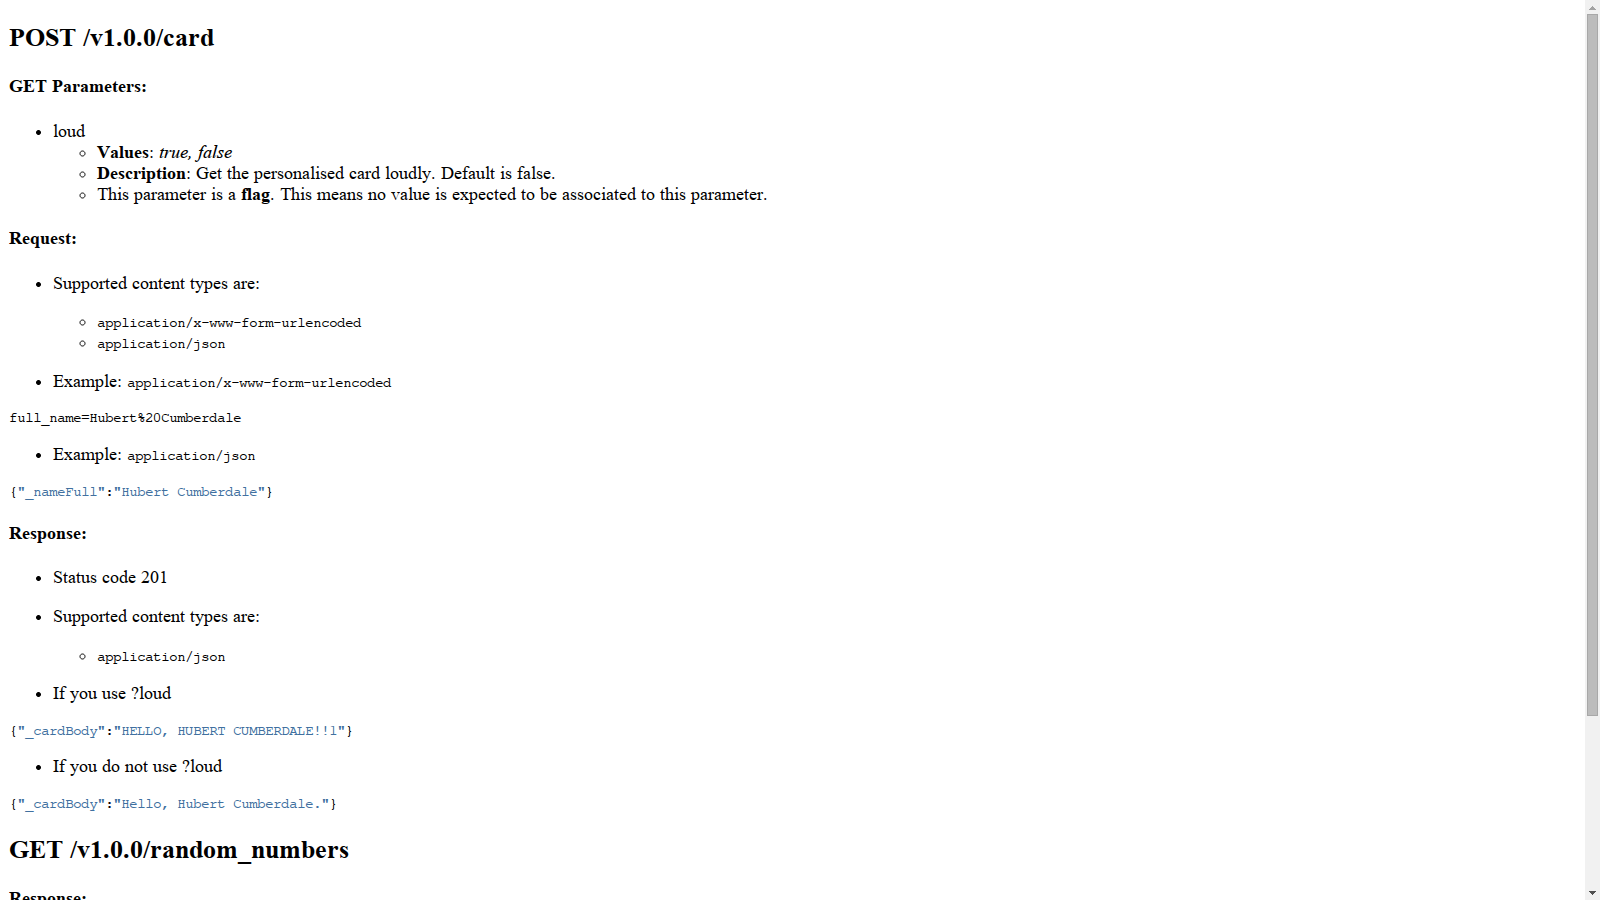
\includegraphics{big.png}
\caption{Auto-generated docs}
\end{figure}

\end{frame}

\begin{frame}{Converted to HTML}

\begin{figure}[htbp]
\centering
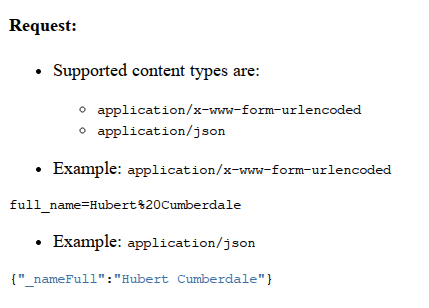
\includegraphics{zoomed.png}
\caption{Auto-generated docs (zoomed to request)}
\end{figure}

\end{frame}

\begin{frame}{Clients for free (tackling complexity)}

Consider an unversioned API that has:

\begin{itemize}[<+->]
\itemsep1pt\parskip0pt\parsep0pt
\item
  Three breaking changes
\item
  Six users
\end{itemize}

How many changes must you make to fix all of the things?

\end{frame}

\begin{frame}{Clients for free (tackling complexity)}

\begin{figure}[htbp]
\centering
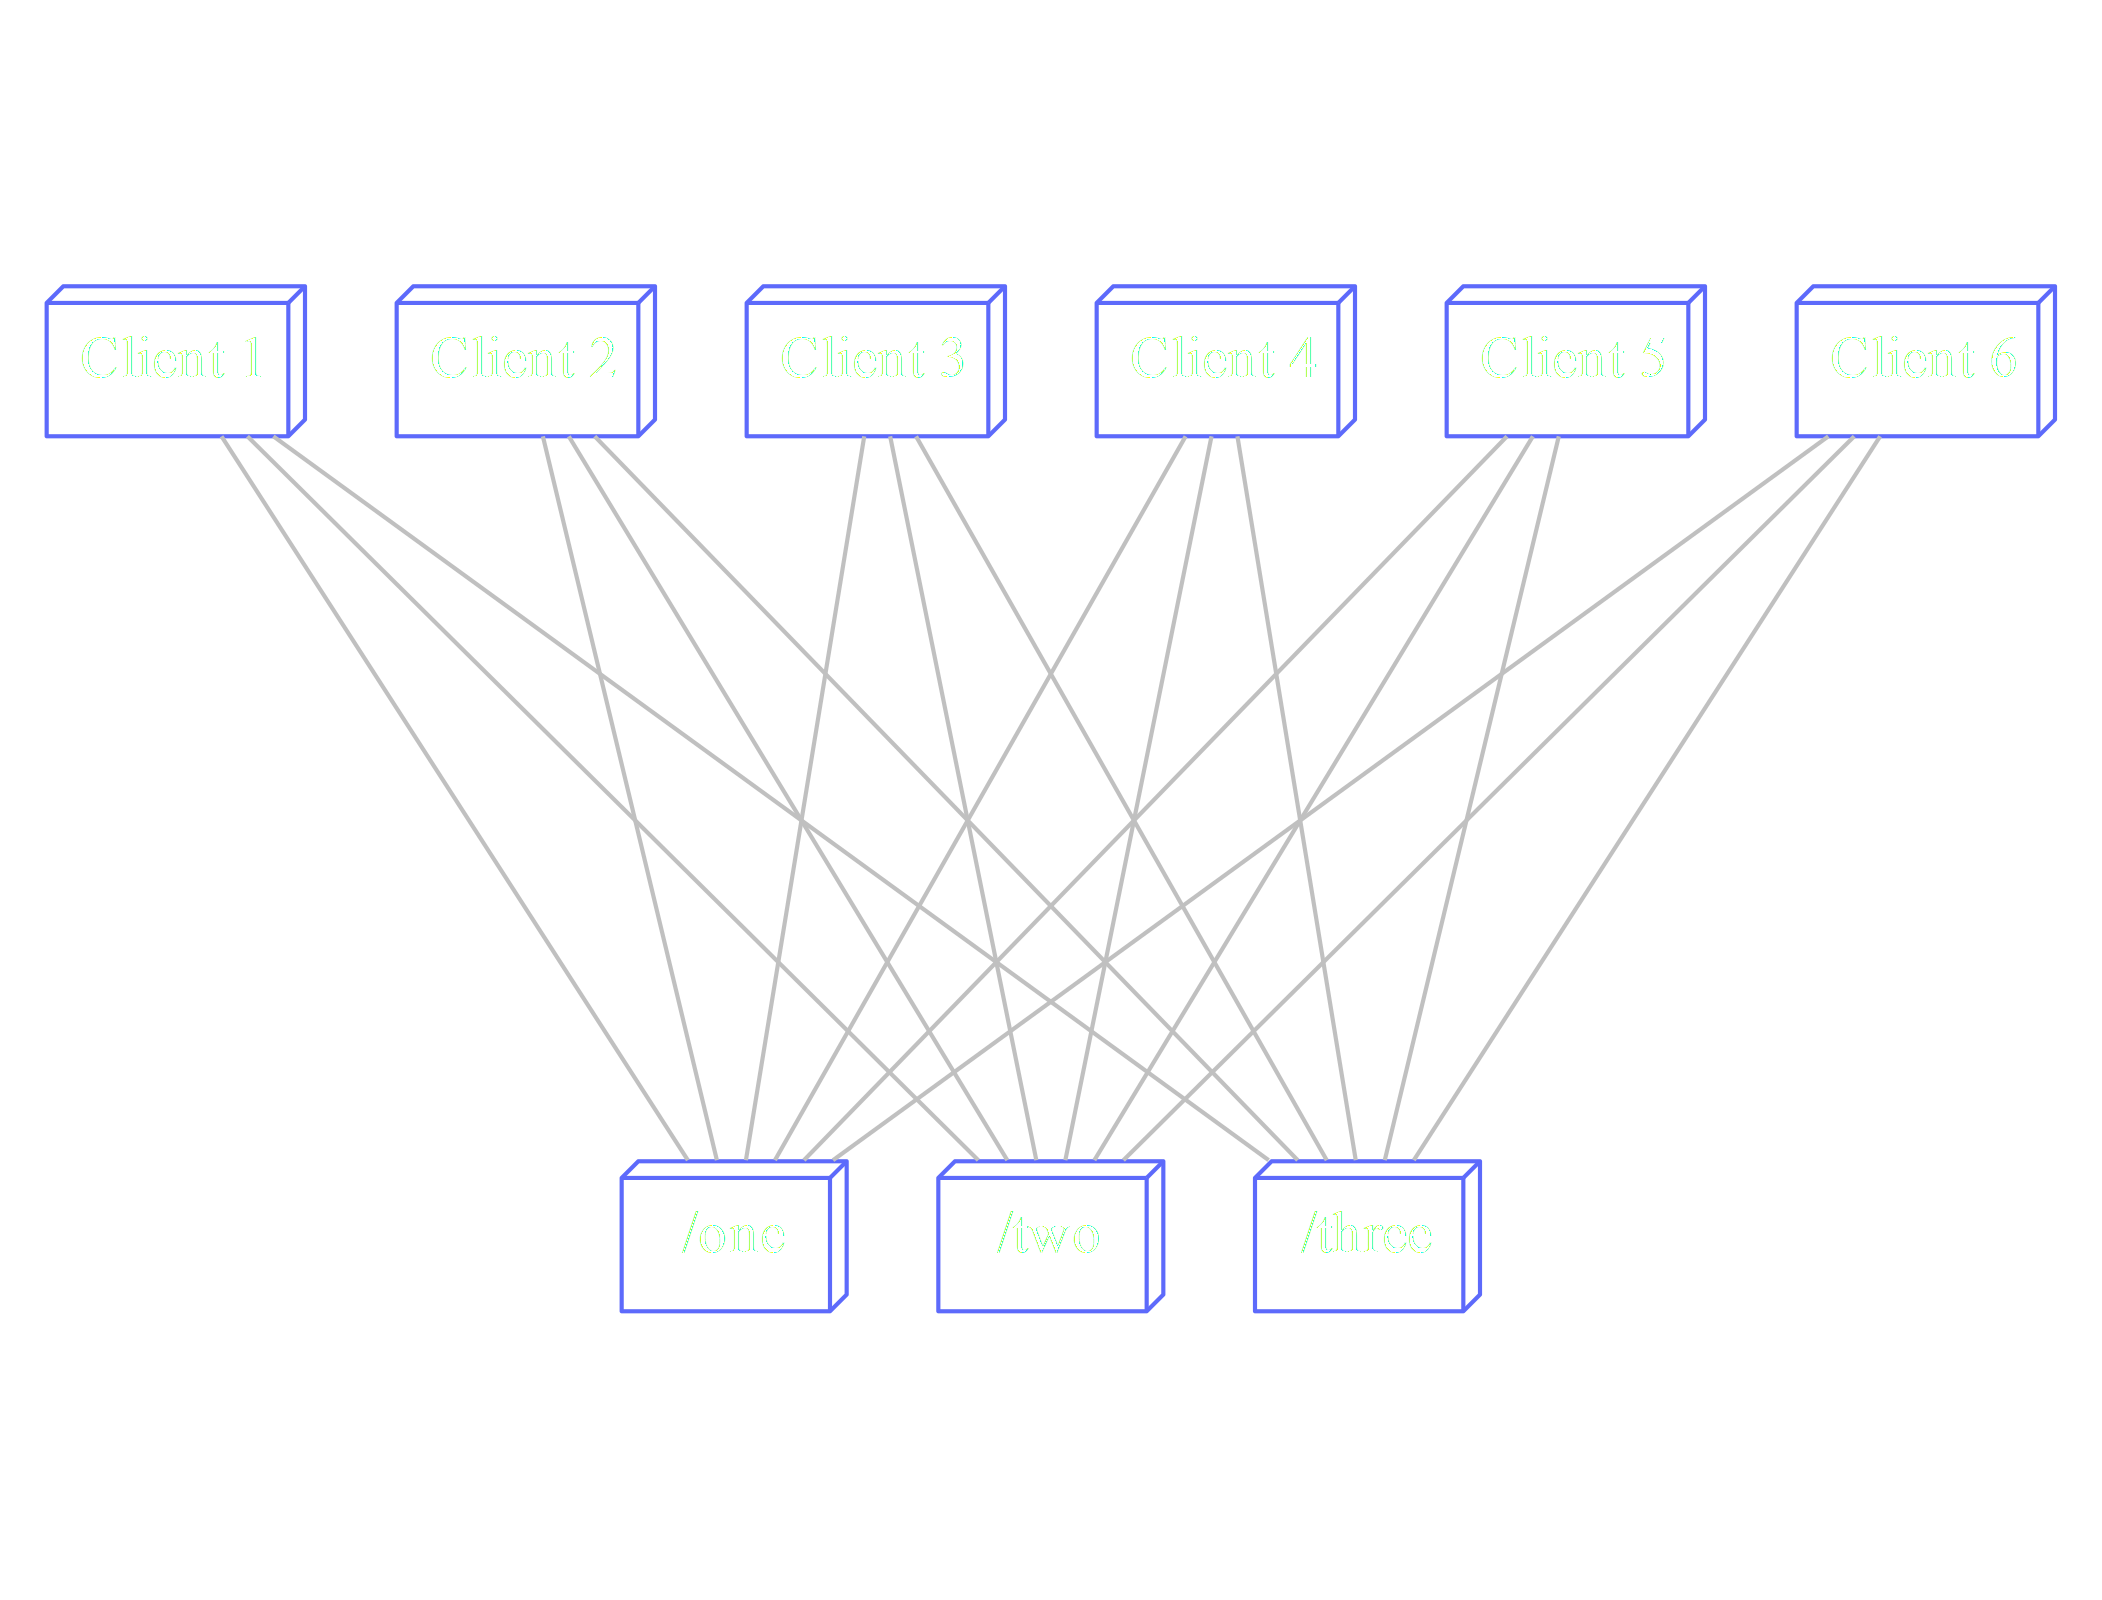
\includegraphics{square.png}
\caption{Complexity to maintain}
\end{figure}

\end{frame}

\begin{frame}[fragile]{Writing clients, the lazy way}

\begin{Shaded}
\begin{Highlighting}[]
\NormalTok{createCard}
\OtherTok{    ::} \DataTypeTok{Bool}
    \OtherTok{->} \DataTypeTok{Name}
    \OtherTok{->} \DataTypeTok{BaseUrl}
    \OtherTok{->} \DataTypeTok{EitherT} \DataTypeTok{ServantError} \DataTypeTok{IO} \DataTypeTok{PersonalisedCard}

\NormalTok{getDice}
\OtherTok{    ::} \DataTypeTok{BaseUrl}
    \OtherTok{->} \DataTypeTok{EitherT} \DataTypeTok{ServantError} \DataTypeTok{IO} \NormalTok{[}\DataTypeTok{Int}\NormalTok{]}

\NormalTok{(createCard }\FunctionTok{:<|>} \NormalTok{getDice) }\FunctionTok{=} \NormalTok{client cardApi}
\end{Highlighting}
\end{Shaded}

\end{frame}

\begin{frame}[fragile]{How could such a magical unicorn exist?}

\begin{Shaded}
\begin{Highlighting}[]
\NormalTok{client}
\OtherTok{  ::} \DataTypeTok{HasClient} \NormalTok{layout }\OtherTok{=>} \DataTypeTok{Proxy} \NormalTok{layout }\OtherTok{->} \DataTypeTok{Client} \NormalTok{layout                     }
\end{Highlighting}
\end{Shaded}

\end{frame}

\begin{frame}[fragile]{The magic: distribute
(:\textless{}\textbar{}\textgreater{})}

\begin{Shaded}
\begin{Highlighting}[]
\KeywordTok{class} \DataTypeTok{HasClient} \NormalTok{layout }\KeywordTok{where}
  \KeywordTok{type} \DataTypeTok{Client}\OtherTok{ layout ::} \FunctionTok{*}
  \NormalTok{clientWithRoute}
\OtherTok{    ::} \DataTypeTok{Proxy} \NormalTok{layout }\OtherTok{->} \DataTypeTok{Req} \OtherTok{->} \DataTypeTok{Client} \NormalTok{layout}


  \KeywordTok{instance} \NormalTok{(}\DataTypeTok{HasClient} \NormalTok{a, }\DataTypeTok{HasClient} \NormalTok{b)}
        \OtherTok{=>} \DataTypeTok{HasClient} \NormalTok{(a }\FunctionTok{:<|>} \NormalTok{b) }\KeywordTok{where}               
    \KeywordTok{type} \DataTypeTok{Client} \NormalTok{(a }\FunctionTok{:<|>} \NormalTok{b) }\FunctionTok{=} \DataTypeTok{Client} \NormalTok{a }\FunctionTok{:<|>} \DataTypeTok{Client} \NormalTok{b                               }
    \NormalTok{clientWithRoute }\DataTypeTok{Proxy} \NormalTok{req }\FunctionTok{=}                                                   
      \NormalTok{clientWithRoute (}\DataTypeTok{Proxy}\OtherTok{ ::} \DataTypeTok{Proxy} \NormalTok{a) req }\FunctionTok{:<|>}                                 
      \NormalTok{clientWithRoute (}\DataTypeTok{Proxy}\OtherTok{ ::} \DataTypeTok{Proxy} \NormalTok{b) req   }
\end{Highlighting}
\end{Shaded}

\end{frame}

\begin{frame}[fragile]{Clients for free!}

\begin{Shaded}
\begin{Highlighting}[]
\NormalTok{createCard}
\OtherTok{    ::} \DataTypeTok{Bool}
    \OtherTok{->} \DataTypeTok{Name}
    \OtherTok{->} \DataTypeTok{BaseUrl}
    \OtherTok{->} \DataTypeTok{EitherT} \DataTypeTok{ServantError} \DataTypeTok{IO} \DataTypeTok{PersonalisedCard}

\NormalTok{getDice}
\OtherTok{    ::} \DataTypeTok{BaseUrl}
    \OtherTok{->} \DataTypeTok{EitherT} \DataTypeTok{ServantError} \DataTypeTok{IO} \NormalTok{[}\DataTypeTok{Int}\NormalTok{]}

\NormalTok{(createCard }\FunctionTok{:<|>} \NormalTok{getDice) }\FunctionTok{=} \NormalTok{client cardApi}
\end{Highlighting}
\end{Shaded}

\end{frame}

\begin{frame}[fragile]{Type safe URLs}

\begin{Shaded}
\begin{Highlighting}[]
\NormalTok{safeLink}
\OtherTok{    ::} \NormalTok{forall endpoint api}\FunctionTok{.} \NormalTok{( }\DataTypeTok{IsElem} \NormalTok{endpoint api}
                            \NormalTok{, }\DataTypeTok{HasLink} \NormalTok{endpoint)}
    \OtherTok{=>} \DataTypeTok{Proxy} \NormalTok{api}
    \OtherTok{->} \DataTypeTok{Proxy} \NormalTok{endpoint}
    \OtherTok{->} \DataTypeTok{MkLink} \NormalTok{endpoint}
\end{Highlighting}
\end{Shaded}

\end{frame}

\begin{frame}[fragile]{With input!}

\begin{Shaded}
\begin{Highlighting}[]
\KeywordTok{let} \NormalTok{nums }\FunctionTok{=} \DataTypeTok{Proxy}\OtherTok{ ::} \DataTypeTok{Proxy} \NormalTok{(}\StringTok{"v1.0.0"} \FunctionTok{:>} \DataTypeTok{RandomInts}\NormalTok{)}
\NormalTok{print }\FunctionTok{$} \NormalTok{safeLink cardApi nums }
\end{Highlighting}
\end{Shaded}

\pause

\begin{verbatim}
>> v1.0.0/random_numbers
\end{verbatim}

\pause

\begin{Shaded}
\begin{Highlighting}[]

\KeywordTok{let} \NormalTok{make_card }\FunctionTok{=} \DataTypeTok{Proxy}\OtherTok{ ::} \DataTypeTok{Proxy} \NormalTok{(}\StringTok{"v1.0.0"} \FunctionTok{:>} \DataTypeTok{MakeCard}\NormalTok{)}
\KeywordTok{let}\OtherTok{ f ::} \DataTypeTok{Bool} \OtherTok{->} \DataTypeTok{URI} \FunctionTok{=} \NormalTok{safeLink cardApi make_card}
\NormalTok{traverse_ print [f }\DataTypeTok{True}\NormalTok{, f }\DataTypeTok{False}\NormalTok{]}
\end{Highlighting}
\end{Shaded}

\pause

\begin{verbatim}
>> v1.0.0/card?loud
>> v1.0.0/card
\end{verbatim}

\end{frame}

\begin{frame}{Conclusion}

\begin{itemize}[<+->]
\itemsep1pt\parskip0pt\parsep0pt
\item
  Types and webservices can be friends
\item
  By defining your API as a type, you can get for free:

  \begin{itemize}[<+->]
  \itemsep1pt\parskip0pt\parsep0pt
  \item
    Server boilerplate
  \item
    Documentation
  \item
    Clients (Haskell, jquery, PureScript)
  \item
    Safe links
  \end{itemize}
\end{itemize}

\end{frame}

\end{document}
